\documentclass[11pt, oneside]{article}   	% use "amsart" instead of "article" for AMSLaTeX format
\usepackage{geometry}                		% See geometry.pdf to learn the layout options. There are lots.
\geometry{letterpaper}                   		% ... or a4paper or a5paper or ... 
%\geometry{landscape}                		% Activate for for rotated page geometry
%\usepackage[parfill]{parskip}    		% Activate to begin paragraphs with an empty line rather than an indent
\usepackage{graphicx}				% Use pdf, png, jpg, or eps� with pdflatex; use eps in DVI mode
								% TeX will automatically convert eps --> pdf in pdflatex		
\usepackage{amssymb}
\usepackage{amsmath}
\usepackage{parskip}

\title{Trig substitutions}
%\author{The Author}
\date{}							% Activate to display a given date or no date
\graphicspath{{/Users/telliott_admin/Dropbox/Tex/png/}}

\begin{document}
\maketitle
%\section{}
%\subsection{}
\Large
Kline has a discussion of rotatation of axes (Chapter 7 A1).  It leads to a method for finding the angle by which to rotate in order to eliminate the $xy$ term in the general equation
\[ Ax^2 + Bxy + Cy^2 + Dx + Ey + F = 0 \]
Start with the rotation formulas.  We rotate the $xy$-axes to $x'y'$ by an angle $\theta$.  Then we consider a point $P = (x,y)$
\begin{center} 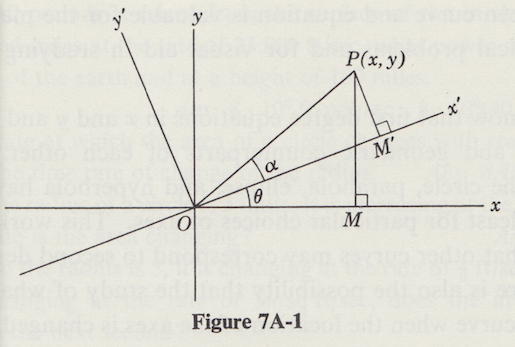
\includegraphics [scale=0.5] {Kline_7A_1.png} \end{center}
Drop a perpendicular to the $x'y'$-axes and form the angle $\alpha$.  We have used a construction like this to derive the sum of angles formulas.  Here, we go over the same ground, but in reverse:
\[ \cos \theta + \alpha = \cos \theta \cos \alpha - \sin \theta \sin \alpha \]
\[ x = OP ( \cos \theta + \alpha) \]
\[ = OP (\cos \theta \cos \alpha - \sin \theta \sin \alpha) \]
\[ =  x' \cos \theta - y' \sin \theta \]
Using the other formula
\[ \sin \theta + \alpha = \sin \theta \cos \alpha+ \cos \theta \sin \alpha \]
\[ y = OP( \sin \theta + \alpha) \]
\[ = OP( \sin \theta \cos \alpha + \cos \theta \sin \alpha) \]
\[ = x' \sin \theta + y' \cos \theta \]
Substituting into the general equation, we obtain a large number of terms including:
\[ Ax^2 = A(x'^2 \sin^2 \theta - 2x'y'\sin \theta \cos \theta + y'^2 \cos^2 \theta) \]
\[ Bxy = B(x'^2 \sin \theta \cos \theta - x'y' \sin^2 \theta + x'y' \cos^2 \theta - y'^2 \sin \theta \cos \theta ) \]
\[ Cy^2 = C(x'^2 \sin^2 \theta + 2x'y' \sin \theta \cos \theta + y'^2 \cos \theta) \]
plus other terms that do not contain $x'y'$.  Gather together those $x'y'$ terms and set the sum equal to zero to make them vanish:
\[ -2A x'y'\sin \theta \cos \theta - Bx'y' \sin^2 \theta + Bx'y' \cos^2 \theta + 2Cx'y' \sin \theta \cos \theta = 0 \]
\[ -2A \sin \theta \cos \theta - B \sin^2 \theta + B \cos^2 \theta + 2C \sin \theta \cos \theta = 0 \]
Employ the sum of angles formulas in a different guise:
\[ \cos 2 \theta = \cos^2 \theta - \sin^2 \theta \]
\[ \sin 2 \theta = 2 \sin \theta \cos \theta \]
We plug into the $x'y'$ formula to obtain:
\[ (C-A) \sin 2 \theta + B \cos 2 \theta = 0 \]
\[ \tan 2 \theta = \frac{B}{A-C} \]
A reassuring simplification.  As an example, for the hyperbola
\[ xy = 1 \]
\[ xy - 1 = 0 \]
$B=1$ and $A=C=0$, for which we simply invert the formula to find that 
\[ \cot 2 \theta = 0 = \cos 2 \theta \]
Hence $2 \theta = \pi/2$ and $\theta = \pi/4$.
For the transformed equation, most terms are zero since $A = C = D = E = 0$.  We are left with only
\[ B( x'^2 \sin \theta \cos \theta - y'^2 \sin \theta \cos \theta ) - 1 = 0 \]
\[ \frac{x'^2}{2} - \frac{y'^2}{2} = 1 \]
which is the rotated hyperbola.

\end{document}  